% Task 1 -- interpretability across boundary conditions. Compile: pdflatex (x2).
\documentclass[aspectratio=169,10pt]{beamer}
\usepackage[T1]{fontenc}\usepackage{lmodern}\usepackage{amsmath,amssymb,bm}
\usepackage{booktabs}\usepackage{graphicx}
\graphicspath{{../../asm_bug_demo/infoprop_out/}}
\definecolor{Struct}{HTML}{1F3A5F}\definecolor{Gray}{HTML}{6E6E6E}\definecolor{Accent}{HTML}{8C2D04}
\usetheme{default}\usefonttheme{professionalfonts}\setbeamertemplate{navigation symbols}{}
\setbeamercolor{structure}{fg=Struct}\setbeamercolor{frametitle}{fg=Struct}
\setbeamerfont{frametitle}{series=\bfseries,size=\large}
\setbeamercolor{block title}{fg=white,bg=Struct}\setbeamercolor{block body}{bg=Struct!6}
\setbeamertemplate{frametitle}{\vskip0.45em\hspace{0.2em}\usebeamerfont{frametitle}\insertframetitle%
  {\ifx\insertframesubtitle\empty\else\\[0.1em]\small\color{Gray}\insertframesubtitle\fi}\par}
\setbeamertemplate{footline}{\hfill\footnotesize\color{Gray}\insertframenumber\,/\,\inserttotalframenumber\hspace{0.4cm}\vspace{3pt}}
\renewcommand{\arraystretch}{1.15}
\begin{document}

% ===== Title =====
\begin{frame}[plain]
\vskip1.1cm
{\color{Struct}\large\bfseries Task 1 --- Interpretability across boundary conditions\par}
\vskip0.4em{\color{Gray} all-Dirichlet vs all-Neumann vs mixed, on the unit geometry (1D/2D/3D)\par}
\vskip0.8em\hrule height0.4pt\vskip0.6em\footnotesize
The over-count $\hat N$ is geometric (BC-free); the BC only perturbs $\lambda_{\min}$;
a coarse space neutralizes it. \quad(\texttt{asm\_bug\_demo/bc\_suite.c})
\end{frame}

% ===== Problem definition =====
\begin{frame}{Problem definition --- the three concrete examples}
\framesubtitle{$-\Delta u=f$ on the unit hypercube $[0,1]^d$, $d{=}1,2,3$; $(2d{+}1)$-point FD, $n$ nodes/axis}
\begin{itemize}\itemsep0.35em
  \item \textbf{(D) all-Dirichlet}: $u{=}0$ on every face. SPD. \emph{This is the existing 1D/2D minimal case.}
  \item \textbf{(N) all-Neumann}: $\partial u/\partial n{=}0$ on every face. \textbf{Singular} --- null space $=$ constants.
  \item \textbf{(M) mixed}: 1 face Dirichlet $+$ $(2d{-}1)$ faces Neumann (the 3D Sys 3 type).
\end{itemize}
\vskip0.3em\footnotesize
Grid: 1D $n{=}256$ (8 subdomains), 2D $64^2$ ($4{\times}4$), 3D $24^3$ ($4{\times}4{\times}4$); overlap $O{=}2$.
BASIC vs sASM additive Schwarz, exact (Cholesky) / ICC(0) subdomain solves, optional Nicolaides two-level;
outer CG to $10^{-8}$. Singular case: constant \texttt{MatNullSpace} (mean-zero RHS, nullspace-aware coarse solve).
\end{frame}

% ===== Comparison figure =====
\begin{frame}{Item-by-item: what the BC changes, and what it does not}
\begin{center}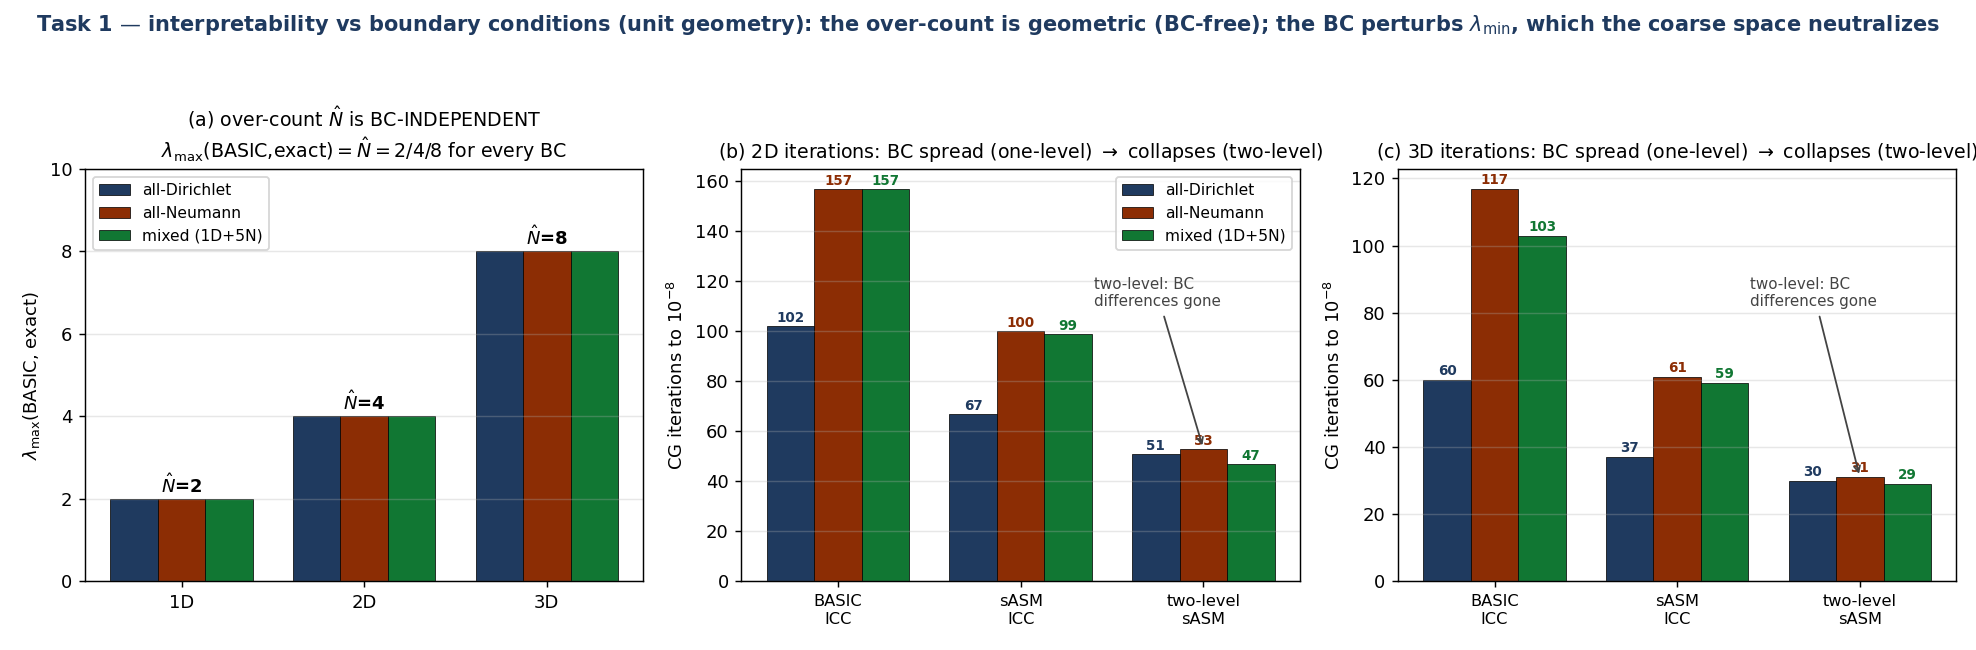
\includegraphics[width=0.99\textwidth]{fig_bc_compare}\end{center}
\vskip-0.2em
\begin{itemize}\itemsep0.04em\scriptsize
  \item \textbf{(a)} the over-count $\lambda_{\max}(\text{BASIC,exact})=\hat N=$2/4/8 is \textbf{identical for all three BC} --- it is geometric.
  \item \textbf{(b,c)} one-level iterations differ by BC (2D BASIC-ICC 102/157/157; Neumann \& mixed are harder); the \textbf{two-level coarse space collapses the spread} (2D sASM 67/100/99 $\to$ 51/53/47).
\end{itemize}
\end{frame}

% ===== The mechanism =====
\begin{frame}{The BC only moves $\lambda_{\min}$; the coarse space neutralizes it}
\begin{block}{Item-by-item summary}
\footnotesize
\begin{tabular}{l ccc l}
\toprule
 & all-Dirichlet & all-Neumann & mixed & BC-dependent? \\
\midrule
over-count $\hat N$ (2D) & 4 & 4 & 4 & \textbf{no} (geometric) \\
$\lambda_{\max}$(BASIC,exact) & $=\hat N$ & $=\hat N$ & $=\hat N$ & \textbf{no} \\
$\lambda_{\min}$ 1-level (2D) & 0.0071 & 0.0039 & \textbf{0.0010} & \textbf{yes} \\
1-level sASM iters (2D) & 67 & 100 & 99 & yes \\
$\lambda_{\min}$ two-level (2D) & 0.045 & 0.053 & 0.043 & \textbf{no} (aligned) \\
two-level iters (2D) & 51 & 53 & 47 & \textbf{no} (collapsed) \\
\bottomrule
\end{tabular}
\end{block}
\vskip0.2em
\begin{itemize}\itemsep0.18em\footnotesize
  \item The BC changes the \textbf{global/constant mode}: Neumann is \emph{singular} (constant null space); mixed is barely pinned by its one Dirichlet face (smallest $\lambda_{\min}$); Dirichlet is best.
  \item \textbf{The Nicolaides PoU coarse space spans the constant} ($\sum_i\phi_i{=}1$) --- exactly the mode the BC perturbs. So it lifts \emph{and aligns} $\lambda_{\min}$ across BC. For all-Neumann the coarse space \emph{is} the null space $\Rightarrow$ the perfect fix.
\end{itemize}
\end{frame}

% ===== Conclusion =====
\begin{frame}{Conclusion (Task 1)}
\begin{itemize}\itemsep0.4em
  \item \textbf{Over-count is BC-free.} $\hat N$ and $\lambda_{\max}(\text{BASIC,exact})=\hat N$ are identical for all-Dirichlet, all-Neumann and mixed --- so the entire sASM ``remove $\hat N$'' story carries over unchanged.
  \item \textbf{The BC only perturbs $\lambda_{\min}$} (the global/constant mode): Neumann singular, mixed near-singular, Dirichlet best $\Rightarrow$ one-level iterations carry a BC spread.
  \item \textbf{A coarse space neutralizes the BC.} Nicolaides (spans the constant) collapses the $\lambda_{\min}$ spread and the iteration spread; for all-Neumann it is the \emph{exact} coarse space (= the null space).
\end{itemize}
\end{frame}

\end{document}
